\documentclass[a4paper,10pt]{article}
\usepackage[utf8]{inputenc}
\usepackage[french] {babel}
\usepackage[T1]{fontenc}
\usepackage{lmodern}
\usepackage{graphicx}
\usepackage{graphics}
\usepackage{ulem}
\usepackage{amssymb}
\usepackage{url}
\usepackage[a4paper]{geometry}
\geometry{hscale=0.7,vscale=0.7,centering}
\usepackage{vmargin}
\usepackage{amsmath}
\usepackage{amssymb}
\usepackage{amsthm}
\usepackage{moreverb}
\usepackage{listings}
\newtheorem{theorem}{Théorème}[section]
\newtheorem{defi}{Définition}[section] 
\newtheorem{prop}{Propriété}[section] 
\usepackage{color}
\definecolor{gris}{rgb}{0.95,0.95,0.95}
\lstset{numbers=left, tabsize=4, backgroundcolor=\color{gris},
frame=single, breaklines=true,
keywordstyle=\color{black},
stringstyle=\ttfamily,
framexleftmargin=6mm, xleftmargin=6mm}
%opening
\title{LINGI 2261 : Artificial Intelligence \\
Assignement 3 - Mid-Project}
\author{Rochet Florentin - Debroux Léonard} 
\date{Année académique 2011-2012}

\begin{document}

	\begin{titlepage}
		\begin{center}
			{\huge LINGI2261: Artificial Intelligence}\\
			\vspace{0.4cm}
			
			{\Large {Professor : Yves Deville\\ \vspace{0.2cm} Teaching assistants : Cyrille Dejemeppe and Jean-Baptiste Mairy  }}\\
			\vspace{0.6cm}
			
			{\Large \textit{ Assignement3 : Adversarial Search}}\\
			\vspace{1.2cm}

			\texttt{}\\
			\vspace{0.2cm}

			
\includegraphics[height=10cm]{pageGarde.png}\\
			\vspace{0.1cm}
			{\Large \textbf{Universit\'e Catholique de Louvain}}
			\vspace{0.7cm}

			Groupe 37 \\
			\vspace{0.2cm}
			
			Florentin Rochet \\
			Léonard Debroux\\
			\vspace{0.2cm}
			2012-2013\\
		\end{center}
	\end{titlepage}

	\newpage
	

	\section{Scipion}
		Here is the tree representing the game of scipion, we also included the representation of the board of the game at each step.
		\begin{figure}[h!]
			\centering
				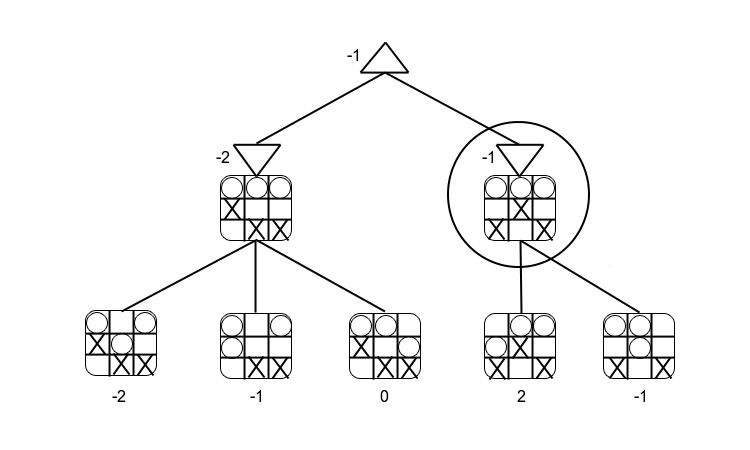
\includegraphics[scale=0.5]{minmax_tree_scipion_specs.png}
			\caption{Scipion Tree}
		\end{figure}\\
		On this tree, we can find at the bottom the values of the leaves. From them are derived the values of the other nodes using minimax. We see that as the root is max, it should play the right action.
	\section{Alpha-Beta search}	
		\subsection{Perform the MiniMax algorithm on the tree in Figure 4, i.e. put a value to each node. Circle the move the root player should do.}
		\begin{figure}[h!]
			\centering
				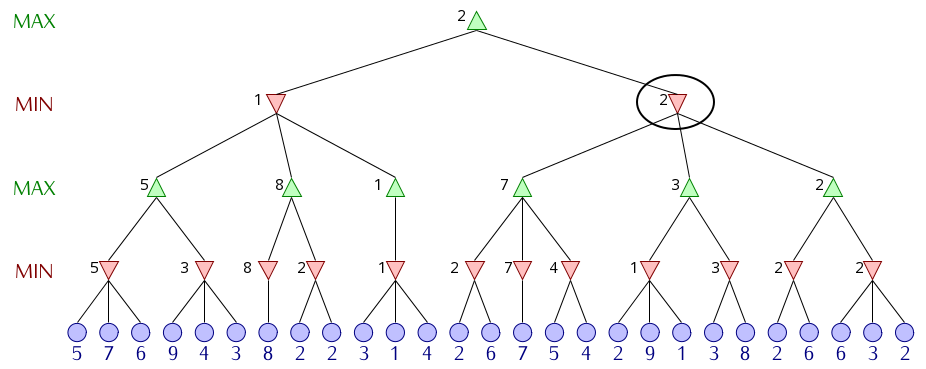
\includegraphics[scale=0.4]{arbre_minimax.png}
			\caption{MiniMax}
		\end{figure}
		The action to be played is thus the one at the right of the root.
		\subsection{Perform the Alpha-Beta algorithm on the tree. At each non terminal node, put the successive values of $\alpha$ and $\beta$. Cross out the arcs reaching non visited nodes. Assume a left-to-right node expansion.}		
		\begin{figure}[h!]
			\centering
				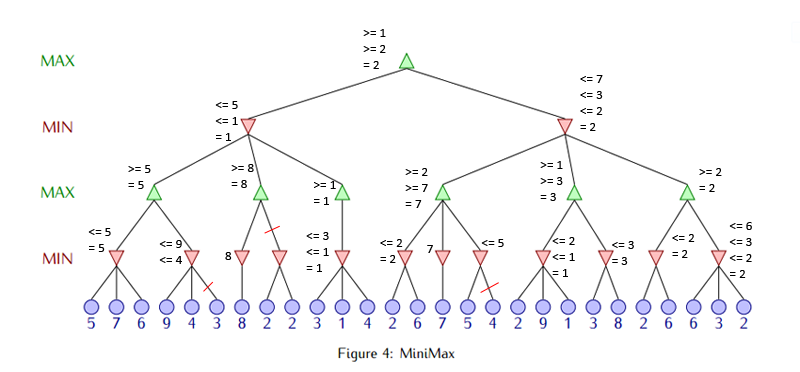
\includegraphics[scale=0.8]{tree-fig5.png}
			\caption{AlphaBeta from left right}
		\end{figure}
		\subsection{Do the same, assuming a right-to-left node expansion instead}
		\begin{figure}[h!]
			\centering
				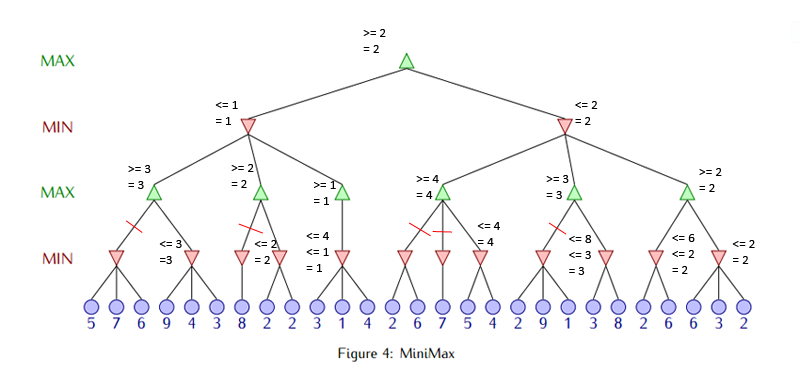
\includegraphics[scale=0.8]{tree-fig6.png}
			\caption{AlphaBeta from right to left}
		\end{figure}
		\subsection{Can the nodes be ordered in such a way that Alpha-Beta pruning can cut off more branches (in a left-to-right node expansion)? If no, explain why; if yes,
give the new ordering and the resulting new pruning.}
		Yes it can. What we have to do is to order the successors of every nodes when creating them. If we compute the children of a min, we must order them in increasing order and if we compute the children of a max, we must order them in decreasing order.
	\section{Sarena}
		\subsection{A basic Alpha-Beta agent}
			The implementation of the basic\_player is given on the svn repository.
		\subsection{Comparison of MiniMax and Alpha-Beta}
			\subsubsection{Question 4: What action will be played when using the MiniMax algorithm and when using the Alpha-Beta algorithm? Is there a difference between both results?}
			The two played actions will be the same because the difference between MiniMax and Alpha-Beta is that the latter uses pruning. The only difference between the two results is that Alpha-Beta will visit less nodes than MiniMax and so, less time is needed.
			\subsubsection{Question 5: For both algorithms, give the time taken and the number of nodes that are visited when searching the tree. Does this meet your expectations?}
				The results of the tests are below. We didn't get to completion by using the MiniMax strategy, the amount of nodes goes past 10M nodes and so, we didn't let the game run long enough to see a result.
				\begin{center}
					\begin{tabular}{|c||c|c|}
						\hline 
						 & \textbf{Time [s]} & \textbf{Nodes} \\ 
						\hline 
						\textbf{MiniMax} & / & / \\ 
						\hline 
						\textbf{Alpha-Beta} & 87.82 & 371,175 \\
						\hline 
					\end{tabular}
				\end{center} 
				This meets our expectations as we first run Alpha-Beta and it already took some time, it is normal that MiniMax takes so much time.

			\subsubsection{Question 6: For both algorithms, report the number of nodes that are visited at each depth level of the tree.a What do you observe? Explain.}
				As we only reached a solution for the Alpha-Beta algorithm here is the number of nodes visited per depth.
				\begin{center}
					\begin{tabular}{|c|c|c|c|c|c|c|c|c|c|c|c|}
						\hline 
						\textbf{Depth} & 0 & 1 & 2 & 3 & 4 & 5 & 6 & 7 & 8 & 9 & 10 \\ 
						\hline 
						\textbf{Nodes} & 1 & 24 & 63 & 659 & 2,113 & 11,427 & 28,131 & 78,554 & 95,481 & 109,704 & 45,018 \\ 
						\hline 
					\end{tabular} 
				\end{center}
				What is worth observing is the obvious result of 24 nodes at the depth 1 which correspond to $ 1*4 + 4*3 + 4*2 $ that is the possible moves per position (center, edge and corner).\\
				Also, we can see that at the depth 10, there is less moves than for the depth 9. That is because some game progressions can lead to only 9 moves to completion.
			
			\subsection{Evaluation function}
				\subsubsection{Question 7: Describe your evaluation function.}
				The evaluation function look for each tower of the board. For each one, it first calculate all the possible actions and create an object Action \footnote{see our class Action}, then it checks if this action is contained in our dictionaries of "mustDo" and "suicide" move. Those dictionaries are used to recognize some patterns that we assume that must be done in the next move. It's a look-forward for some precise case. A weight is associate in each of those pattern\footnote{see the action again} and this weight is part of the score. The weight is positive for mustDo and negative for suicide.\\
After, we compute the points associate to each coins that are lost or won. The points are positive for won coins and negative for the lost coins. Those points are add to the score.
And finally, the function counts the numbers of yellow coins and red coins that are, first on bottom of towers located on blank cases and second on top of towers located on arrows cases. The value (yellowCoins-redCoins) is added to the score, which gives the final score.\\
A positive score indicates that we are winning and a negative one tells us that we are losing.

				\subsubsection{Question 8: In Alpha-Beta, the evaluation function is used to evaluate leaf nodes (when the cut-off occurs). As seen in previous questions, the pruning of Alpha-Betadepends on the order of the successors. Explain how your evaluation function could be used to (we hope) obtain more pruning with Alpha-Beta. Are there any drawbacks to your approach?}
					The evaluation function can be used at each state that we compute to order the children of a given node. The order is increasing of decreasing following the parent (min or max).\\
					This increases the chance to have pruning and so, less nodes need to be visited.\\
					The drawback of this is the computation time to perform the sort. We run a few tests, and saw that it was better to avoid doing the sort because the gain in pruning was not worth the time spent ordering.
					The pruning in our implementation comes mostly from the cutoff function that returns True when detecting a suicide action.
				\subsubsection{Question 9: Make an agent using the successor function of the basic player (section 3.1), using your new evaluation function and cutting the tree at its root to use the evaluation function on its direct successors (you can achieve this by making cutoff always return True). Let this agent play against another similar agent using Board.get\_score as evaluation function. Try out multiple matches and vary who plays first. How well does your evaluation function fare?}
					To test this, we launched 40 games, 20 began by the player using our evaluation function and 20 began by the basic\_player.
					\begin{center}
					\begin{tabular}{|c|c|c|c|}
						\hline 
						 & New Eval Begin & Basicplayer begin & Total \\ 
						\hline 
						Won by eval & 15 & 8 & 22 \\ 
						\hline 
						Won by basic & 5 & 11 & 17 \\ 
						\hline 
						Draw & 0 & 1 & 1 \\ 
						\hline 
						\end{tabular} 
					\end{center}
					We see that our successor function is better than get\_score.
			\subsection{Successors function}
				\subsubsection{Question 10: Give an upper bound on the number of successors for one state.}
					There is at most 120 possible actions on one board, we can easily convince ourselves that this is the very first state that allows the most actions. Then, we count how many possible actions for each coin which gives $4*2+4*4*3+4*4*4$ ($4$ corners, $4*4$ edge coins and $4*4$ center coins).
				\subsubsection{Question 11: From random games (at least 100), compute the average number of possible
actions at each step of the game. Plot the results in a graph. What do you observe?}
					Here is the graph generated :
					\begin{figure}[h!]
						\centering
							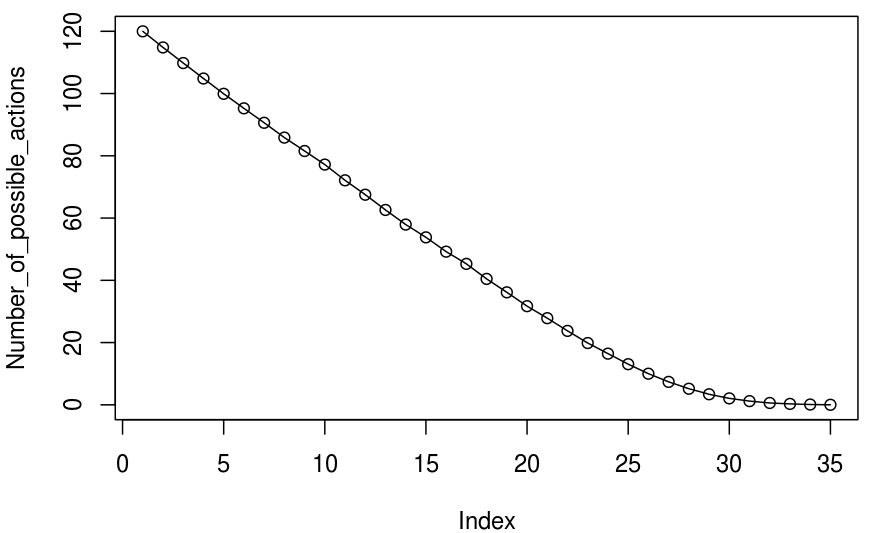
\includegraphics[scale=0.4]{GraphPossActions.png}
						\caption{Number of possible actions per step}
						\label{fig:server_connection}	
					\end{figure}
					We can observe that for the 25 first steps, the decrease is linear. The reason why it stop the be linear between the 25th and the 35 steps is because all games do not reach that much steps.
					
				\subsubsection{Question 12: Are all these successors necessary to be exhaustive (think about symmetry)? Why? If not, how will you consider only the necessary states?}
					There can be symmetrical states:\\
					If we have two independent action $a$ and $b$, the traces $a\rightarrow b$ and $b\rightarrow a$ lead to the same state, so it is unnecessary to treat it twice.\\
					The way to deal with those states is to add a dictionary containing all the visited states for one step of the game. When an action leads to a state that is already in it, we simply don't yield it.
				\subsubsection{Question 13: If the number of successors is still too large, can you think of states that might be ignored, at the expense of loosing completeness?}
					Yes, there are some "suicidal" actions that a normal player wouldn't do because they would lead to certain defeat. We can assume that the opponent won't play "his suicidal action" and we don't want our AI to perform its own "suicidal actions". Thus, we can simply avoid to expand those actions. This detection is done in the cutoff function.
				\subsubsection{Question 14: Describe your successors function.}
					Our successor gets all the possible actions from a state, and only keeps the asymmetrical ones. After that, it simply yields the kept actions. As told before, we could have ordered the successors at this point, but the experience showed that it took way to much time.
				\subsubsection{Question 15: On average, how deep can you explore the tree made by your successors function starting from random initial states (as generated by the constructor of the Board class) in less than 30 seconds? Use an Alpha-Beta agent with the basic evaluation function and increase progressively the cut-off depth.}
					When using only our evaluate, we get the following result for the depths 1, 2 and 3. Those times are an mean on five tries.
					\begin{center}
						\begin{tabular}{|c|c|}
						\hline 
						Depth & Time Taken [s] \\ 
						\hline 
						1 & 0.07712 \\ 
						\hline 
						2 & 0.5748 \\ 
						\hline 
						3 & 20.72 \\ 
						\hline 
						\end{tabular} 
					\end{center}
					Trying a depth of 4 took too much time (more than a minute), so we didn't try to find how much time was needed.\\
					What we can see is that the whole tree of depth 3 is visited in 30 seconds and also the beginning of the forth level is visited.
				
			\subsection{Cut-off function}
				\subsubsection{Question 16: The cutoff method receives an argument called depth. Explain precisely what is called the depth in the minimax.py implementation. Illustrate on an example (draw a search tree and indicate the depths).}
					When drawing the tree of the search, the depth is the level on which we are. It represents in the minimax algorithm the number of action we see in advance. In other words, for a depth d, it means that we have though of all the actions schemes in a range of d actions.\\
					\begin{figure}[h!]
						\centering
							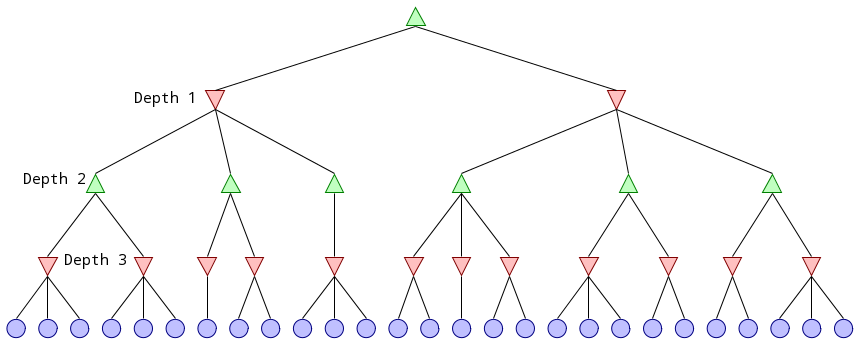
\includegraphics[scale=0.4]{arbre_depth.png}
						\caption{Depth of a minimax tree}
					\end{figure}
				\subsubsection{Question 17: Explain why it might be useful (for the Sarena contest) to cut off the search for another reason than the depth.}
					There is two other reasons than depth to cut the search in our case. the first one is the time that is taken to perform the search and the second one is the detection of the suicides as we want to avoid computing their children.
				\subsubsection{Question 18: Describe your cut-off function.}
					Our cut-off function works in three phases, the first is checking if there is enough time remaining, typically, if only 15 seconds or less remains, we just return True.
					Then, given enough time is left, we check if the action considered is a suicidal move, if yes, it returns True.\\
					And finally, if the search took too much time, based on a maxtime computed with the time\_left and the current step, we decrease the depth of the next search, or, if not, we increase it.\\
					The way it works is by setting a boolean variable to True if a time-out has occurred and when the search is over, we decrease or increase the depth of the next search following the value of the flag.
\end{document}